\chapter{Related Work}

\section{2D and 3D Visualizations}
\label{chap:rw-2d3dLayout}
Although the focus of this thesis is on visualizing hierarchical networks in virtual reality, many concepts are the same or similar to its 2D or 3D counterparts. First we want to give a brief overview of related 2D and 3D approaches in the field of network visualization.\\
Dynamic network visualization describes a research field where none or only few assumptions about the data are made, these techniques often employ force-based layouts using node-link diagrams as we already summarized in the background Section \ref{exp:force_based_background}. Furthermore, we want to discuss approaches dealing with hierarchical and multilayer structured datasets.

\subsection{Hierarchical Visualizations}

As we read in Section \ref{exp:tree}, a preferred data structure to encode hierarchical information are trees.
Schulz \cite{schulz_treevisnet_2011} presented a good overview of different tree visualization techniques. A rough separation can be made by the representation of edges witch is either explicit or implicit. 

\subsubsection{Explicit approaches}
On explicit visualizations, links are directly drawn as we have already seen in \ref{fig:simple_tree}. This core technique is used in numerous application domains and scientific fields. Based on that concept, researchers have developed many extensions to this approach.
LensTree \cite{song_lenstree_2006} for example, exchanges the axes and allows collapsing certain parts of the tree to display information structures like computer file directories. 
Armando et al. \cite{arce-orozco_radial_2017} uses radial instead of parallel axes to show the hierarchical relation. The root node is placed in the center and child nodes extend to all directions along the radius.
Munzer \cite{munzner_h3_1997} extends the radial axis by a third dimension and displays the tree in the 3D hyperbolic space.
Robertson et al. \cite{robertson_cone_1991} also make use of the 3D space for creating a so called cone-tree and cam-tree. These display the child nodes as a circle below or beside their parents.  

\subsubsection{Implicit approaches - space filling}
Space filling approaches use the concept of nesting, which we also use in our layout. In addition, these approaches can encode a value property of the node by the size of the node as we have already seen in Figure \ref{fig:hierarchicalCirclePlot}.
Shneiderman \cite{shneiderman_tree_1992} presented this approach 1992 in the form of a tree map where he visualized the required disk space distribution of a file system. In addition to a common circle packing algorithm \ref{fig:hierarchicalCirclePlot}, Görtler et al. \cite{gortler_bubble_2018} developed a bubble tree map technique, which optimized the used space and allows encoding of additional properties via various shapes, draw strokes and colors. Sunburst charts are another common space filling technique to display node sizes in tree structures. 
As for 3D representations, Wang et al. \cite{wang_visualization_2006} show a circular tree map extended to the z-axis using cylinders. Instead of cylinders, Balzer and Deussen \cite{balzer_hierarchy_2004} use nested hemispheres to visualize software structures.
Other works addressed the performance of layout techniques like Itoh et al. \cite{itoh_hierarchical_2004}, they presented a performance optimized technique for generating a rectangle packing tree map.

The previous presented works show that there are many approaches with various explicit and implicit layouts for tree visualizations. These visualizations focus on mapping hierarchical relationships only. 
However, with our approach we also want to support data structures including links between all kind of nodes not only these covering hierarchical relationships. As long as the connected nodes have the same depth. These data structures are not supported by the presented approaches since this would create a cycle in the original data and therefore breaking the definition of a tree structure in the first place.

\begin{figure}[!hbt]
    \centering
    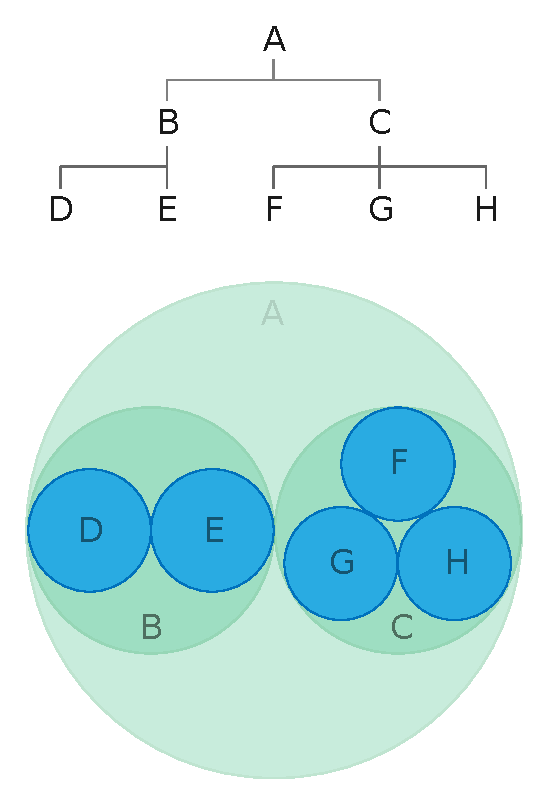
\includegraphics[width=0.40\textwidth, trim={0 0 0 4.3cm},clip]{graphics/circle_packing.pdf}
    \caption{Hierarchical circle packing plot \cite{ribecca_circle_nodate}}
    \label{fig:hierarchicalCirclePlot}
\end{figure}

\subsection{Multilayer Visualization}
We already mentioned in Section \ref{exp:multilayer}, the interesting part of multilayer visualizations is that they enable us to model relationships between multiple separate networks, which are not explicitly supported by the common node-link and tree visualization techniques we discussed before.\\
Domenico et al. \cite{de_domenico_muxviz_2015} presented their MuxVis Toolkit, an open-source software which is able to present multilayer datasets. It provides various layouts (see Figure \ref{fig:muxVisExample}), like a classical stacked one-line layer, a multi-line layer where multiple stacked layer planes are displayed beside each other, a force directed method, and lastly a matrix layout. Besides these so-called 2.5D approaches, there are also classical 2D node-links networks, for example Ducruet \cite{ducruet_multilayer_nodate} display multiple networks showing marine traffic in a single graph just coded by color. 
A combination of multilayer graphs and hierarchical information can be seen in the approach by Eades and Feng \cite{eades_multilevel_1997}, here the authors group the nodes into nested clusters. These are then displayed with a classical multilayer approach as flat layers below each other. The difference to general multilayer graphs is that each node has exactly one connection to its (parent) node in the higher layer. 
Later on, Balzer and Deussen \cite{balzer_level--detail_2007} (see Figure \ref{fig:clusteredGraph}) created a similar visualization but instead of flat layers they used compact 3D surfaces to cluster and group their nodes. Their approach is similar to ours as it also allows nesting multiple levels of nodes and clusters, however they do not have a strict hierarchical aspect. 
Jonker et al. \cite{jonker_graph_2017} uses a level of detail approach where they group parts of the graph into clusters and only display single nodes when zooming into a specific tile. With their 2D layout, they are able to visualize huge networks with multiple hundred thousand nodes and links.
Archambault et al. \cite{archambault_grouseflocks_2008} showed us a visualization approach combining the implicit space filling technique with a hierarchical multilayer network. Their GrouseFlocks system provides  interactive methods to create multiple hierarchical perspectives on the data.  

\begin{figure}[!hbt]
    \centering
    \begin{subfigure}[b]{0.75\columnwidth}
        \centering
        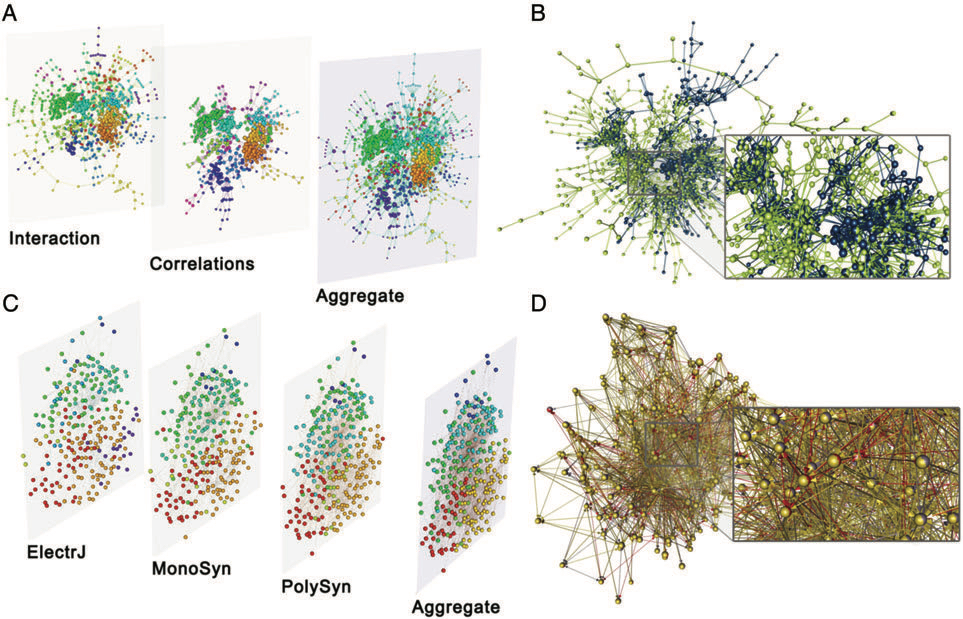
\includegraphics[width=\textwidth]{graphics/muxVisExample.jpg}
        \subcaption{Different supported layout techniques by MuxVis \cite{de_domenico_muxviz_2015}. }
        \label{fig:muxVisExample}
    \end{subfigure}
    \begin{subfigure}[b]{0.45\columnwidth}
        \centering
        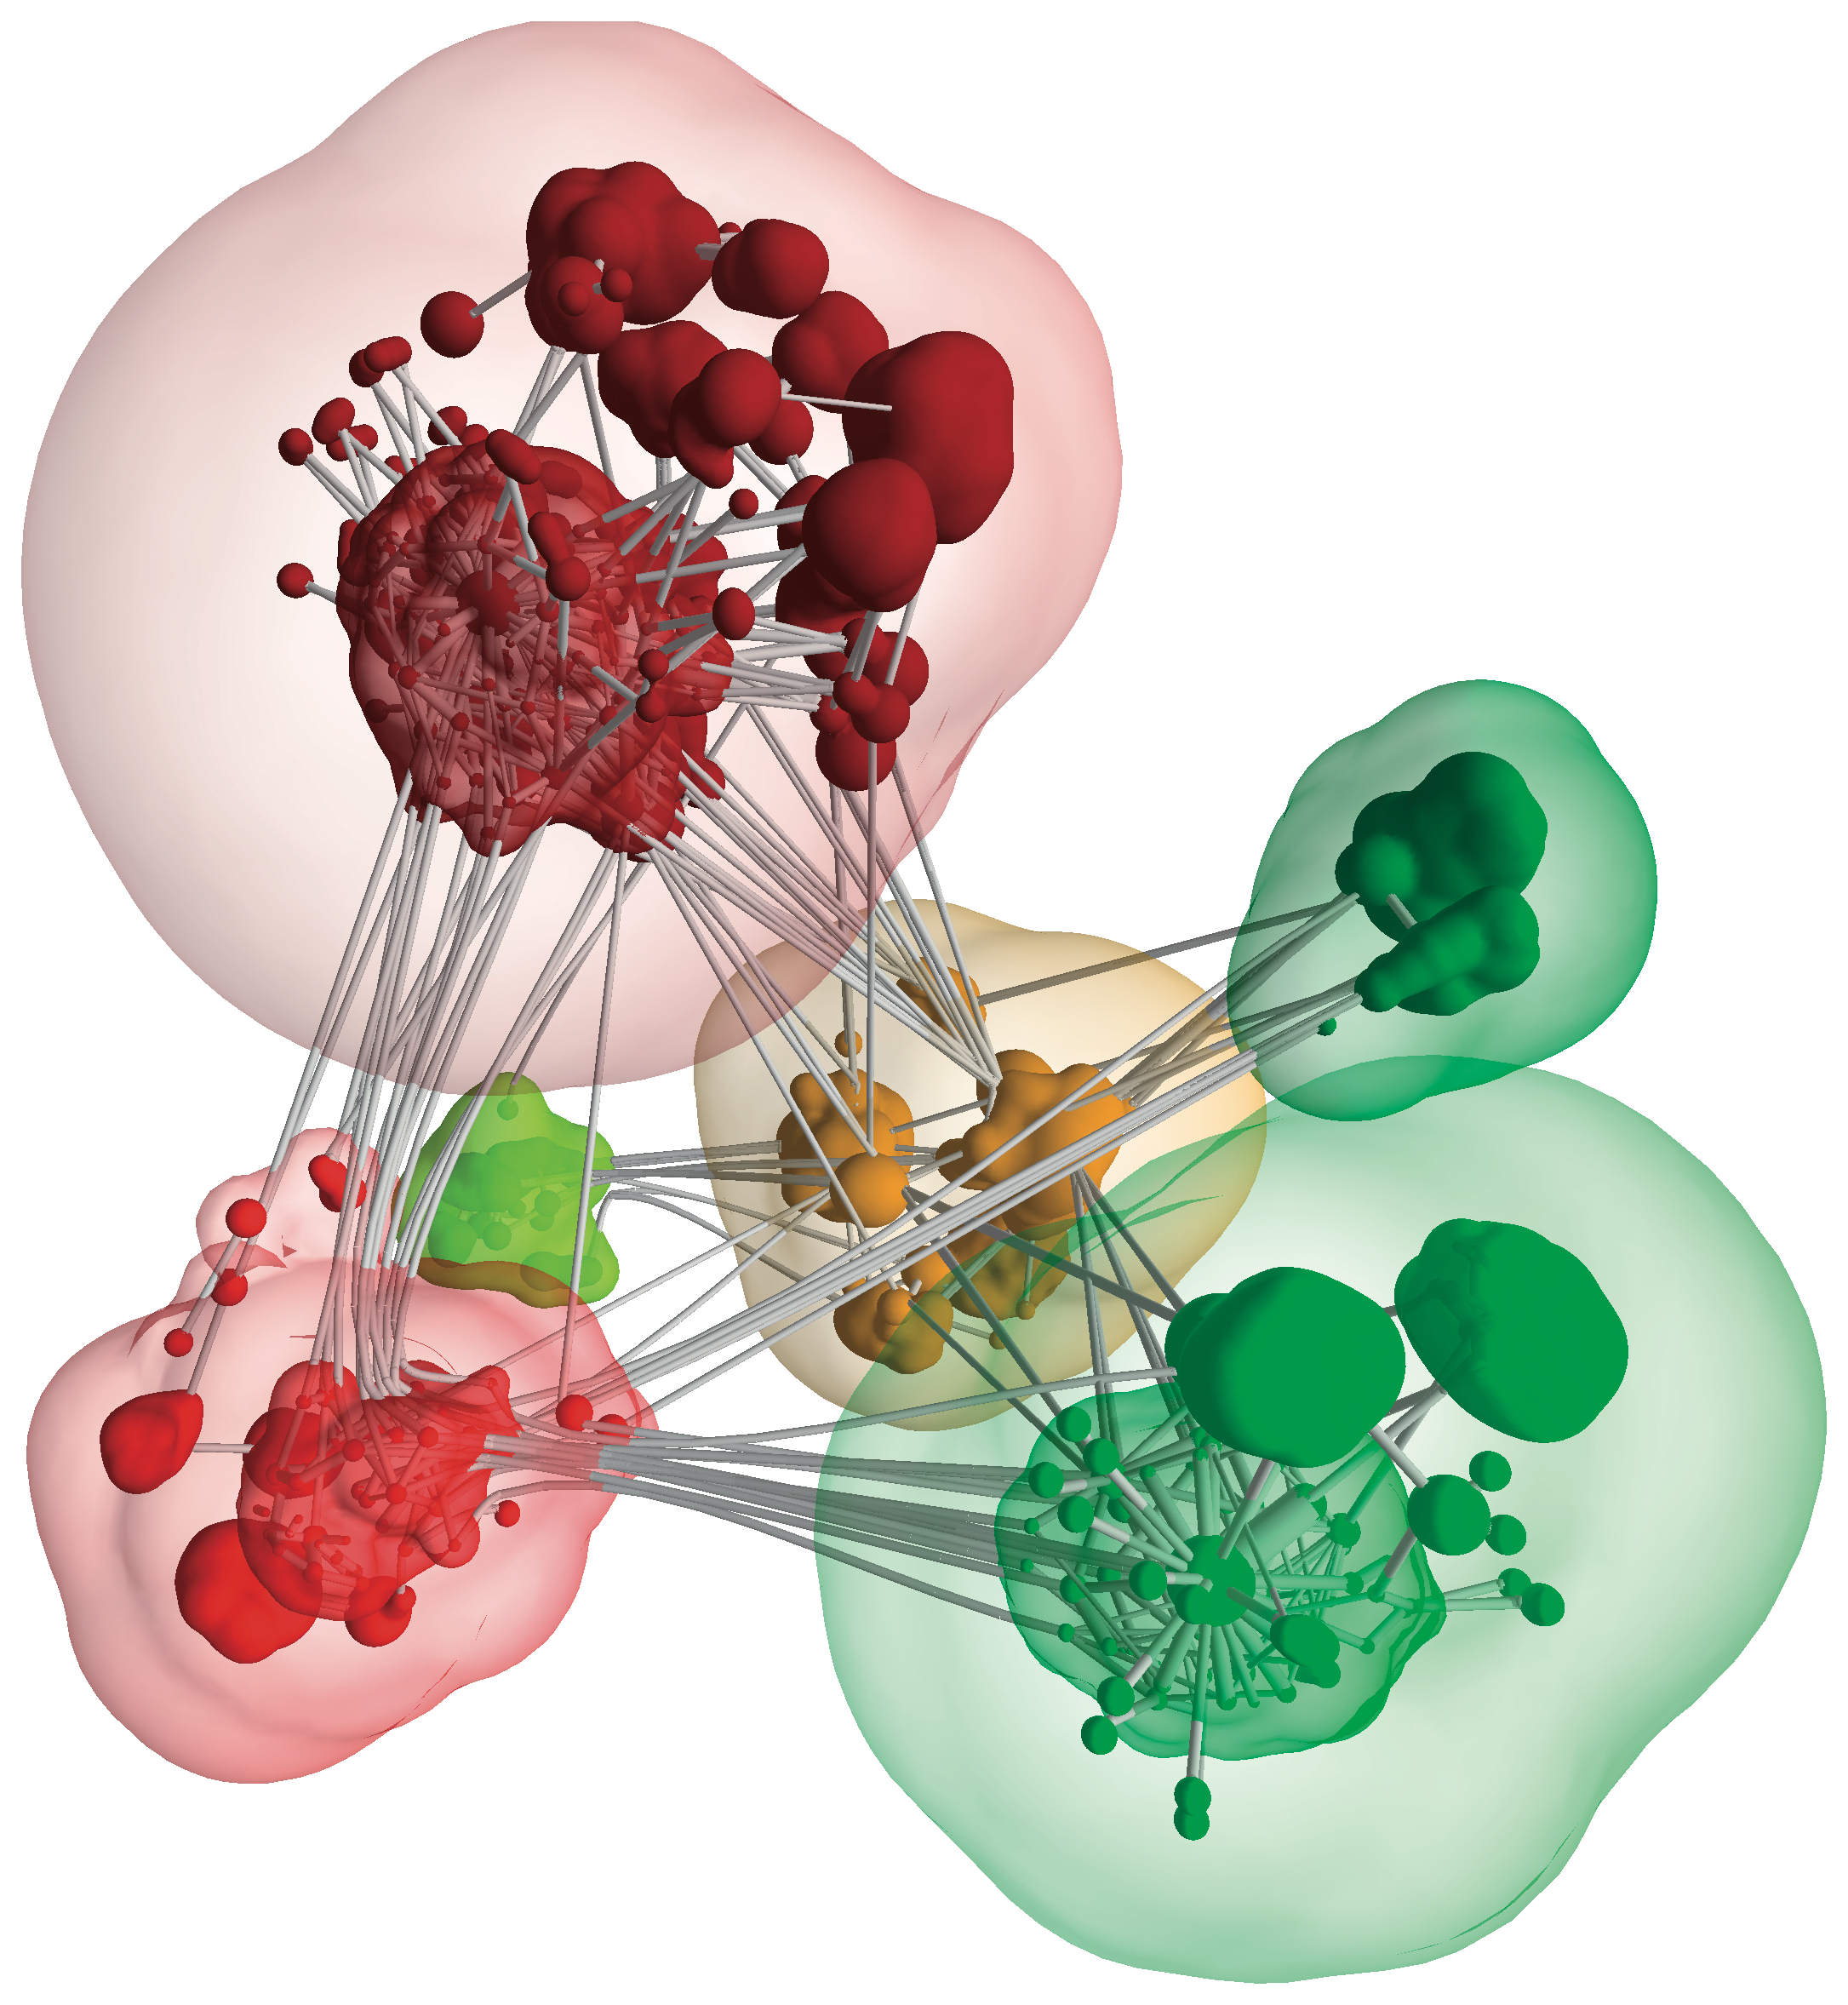
\includegraphics[width=\textwidth]{graphics/clusteredGraphVis.jpg}
        \subcaption{Visualization of a node-link dataset with multiple clusters from \cite{balzer_level--detail_2007}.}
        \label{fig:clusteredGraph}
    \end{subfigure}
    
    \caption{Examples of multilayer visualizations.} % Remove the [...] argument if the original caption should be used in the figure list.
    \label{fig:relatedWorkExamples} 
  \end{figure}

\section{VR Visualizations}
\label{chap:rw-VRVIS}
\subsection{Layouts}
\label{chap:rw-vrlayouts}
In VR, we see common 2D and 3D layout approaches like simple node-link diagrams adapted for the use in a 3D virtual scene. 
Some VR visualizations use a classical spring force layout to calculate their node positions \cite{drogemuller_examining_2020} \cite{sorger_immersive_2019}.
In other visualizations, the position of the nodes comes directly from the data, for example Yang et al. \cite{yang_embodied_2020} use the t-SNE method from Maaten and Hinton \cite{maaten_visualizing_2008} to map the data attributes directly to x, y and z coordinates and display them as a point cloud scatter plot.
In addition to adapted layouts, we also see some new ones specifically designed for the use in VR. Kwon et al. \cite{kwon_study_2016} presented a layout, which displays all nodes on the surface of a sphere. The user stands inside the sphere and is therefore able to freely look around the visualization. Another approach was presented by Halpin et al. \cite{halpin_exploring_2008}. Here the authors display the network on a flat 2D plane in front of the viewer. Through interaction, nodes can be extruded from the flat layout and highlighted on a separated layer.     

\subsection{Navigation}
\label{chap:rw-vrnavigation}

The possibilities for navigation techniques in VR scenes, also called locomotion, depend on the target platform and intended experience the application is built for. As already described in Section \ref{exp:vr-experience}, there are seated-, standing- and room-scale experiences differentiated by the used tracking technologies and the required space.
In seated experiences, the user is usually in front of a normal office desk setup while wearing the head mounted display. Therefore, real world movement is basically no option. 
Standing VR setups normally do not restrict movement, but the users available space to move is extremely limited. Rotating, leaning and hand movement should be supported, but the application can not require the user to walk around.
In room-scale VR setups, the available space can differ greatly. For example HTC Vive requires the user to have a minimum space of $2m * 1.5m$ while a maximum (with 4 base stations) of $10m * 10m$ is possible. As a general rule of thumb, more available space provides more possibilities because the user can navigate through the scene just by walking. 
VR treadmills in theory provide infinite available space to walk, however they are rare and expensive, therefore not suited for our purposes. The conclusion of a study by Usoh et al. \cite{usoh_walking_1999} emphasizes the importance of walking inside a virtual scene. They found that real walking provides a better immersive experience than virtual walking, such as a treadmill would provide and especially better than flying through the scene. 

In most scenarios, however, our virtual scene is bigger than the available space in the real world, therefore we need techniques to navigate through and scale the scene. For seated experiences, Zielasko et al. \cite{zielasko_remain_2017} developed a method that uses a virtual accelerator pedal tracked by a smartphone in the user's pocket and another by leaning the head back and forth. These interactions are then are used to fly through the scene. Similar to the leaning approach, Nguyen-Vo et al. \cite{nguyen-vo_simulated_2018} presented a technique which enables leaning with the chair while seated. To achieve that, they simply used a swopper chair placed onto a Nintendo Wii Balance board, which is able to track the direction of leaning by the distribution of weight.  
Drogemuller et al. \cite{drogemuller_examining_2020} summarized common navigation technique used by various VR applications. One of them is free flying using either gaze direction or the direction where the controller is pointed towards. Often free flying/walking is performed with the left controller while the right can be used for rotating the view without physical rotation, this is especially useful as users often interfere with the cable of the headset while rotating. Another use of the second controller is to describe a direction vector for free flying with the help of the other controller, this is called two handed flying.\\
We can see many approaches that use a free flying technique, however the problem is that many users, especially those new to VR, experience motion sickness, in the context of VR also called cybersickness \cite{zielasko_remain_2017}.
To reduce the effect, a reduction of the field of view while flying with a smooth in and out transition is used by various papers and also often already implemented in common VR frameworks.\\
Beside flying, teleportation is among the most used navigation techniques. Usually the user can point at a location and then press a button to teleport to that position.
This has the advantage of reduced motion sickness because of the reduced animated movement. The challenge of teleportation is to select a suitable point in three-dimensional space without any object nearby. While some approaches solve this with an adjustable teleportation range, Lee et al. \cite{lee_evaluating_2020} present a method to calculate the traveling distance based on the density of the area. In a sparse environment with fewer objects nearby, the distance is higher than in a dense environment with many objects.\\
Worlds-in-Miniature (WIM) \cite{drogemuller_examining_2020} takes the concept of a “minimap” from 2D visualizations into VR by displaying the entire graph in a small scale onto an object near the user, for example the top of the left or right controller. The user can move and rotate the miniature, then select a point with the other controller, which can be mapped to the position of the real graph and furthermore be used for various interaction possibilities like teleporting. Yang et al. \cite{yang_embodied_2020} show us that locomotion can also be achieved via zooming and rotating. They use both controllers to scale, rotate and translate the entire graph at the same time, similar to the zooming and panning used in touch screen applications. This allows the user to freely position the graph and therefore implicitly move around.

\subsection{Interaction}
\label{chap:rw-vrinteraction}

Depending on the application context, there are different goals for interacting with the virtual scene. For visualizations, selection of details, filtering and brushing is important as we already summarized in the information seeking mantra (see Section \ref{seeking mantra}) before. To achieve a precise selection in the scene, researchers have come up with different interaction techniques. The most basic approach to select nodes in the graph would be an infinite ray cast based on the controller direction. To display the detail of the selected node or other selected entity, a head-up display or popup can be used. 
For filtering, Drogemuller et al. \cite{drogemuller_vrige_2017} presented an interesting concept of a filter cube (see Figure \ref{fig:vrFilterCube}). The cube is mapped to an additional Vive tracker, the buttons and sliders on it are used as a virtual input device activated via a virtual click on the button by a controller. 
The concept of a virtual toolbox or gadgets to interact with the environment however is not new. Similar approaches have been implemented in different VR games and creative applications for example Google Blocks VR or Tilt Brush by Google. Switching between multiple tools can be achieved by simply grabbing them with a controller or putting them back in their slot or virtual bag.\\
In addition to the classical controller tracked interaction possibilities, recent achievements in hand tracking technology make hand tracking without any additional equipment possible as new VR headsets, for example the Oculus Quest, come with built in hand tracking. Besides built in technologies, there are also additional sensors available that can be attached to the VR headsets like the Leap Motion Controller. Yi-Jheng Huang et al. \cite{yi-jheng_huang_gesture_2017} used this sensor to build a complex hand gesture system especially designed for the manipulation of a node-link graph in VR. Their gestures can be seen in Figure \ref{fig:vrHandGestures}. 

\begin{figure}[h]
    \centering
    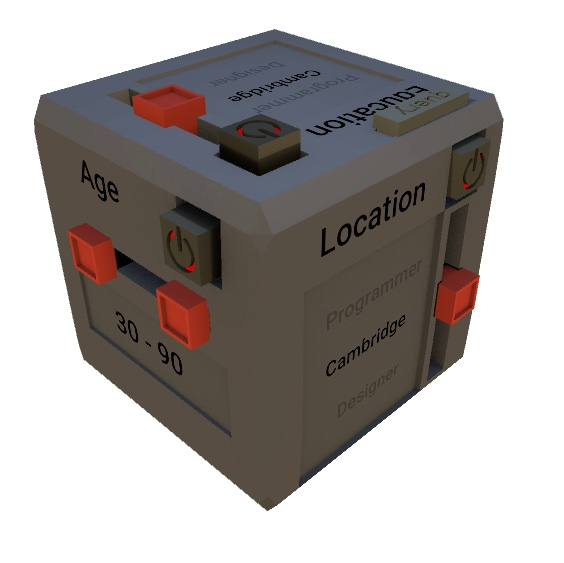
\includegraphics[width=0.4\textwidth]{graphics/filterCube.jpg}
    \caption{Filter cube of Drogemuller et al. \cite{drogemuller_vrige_2017}} 
    \label{fig:vrFilterCube} 
\end{figure}

\begin{figure}[h]
    \centering
    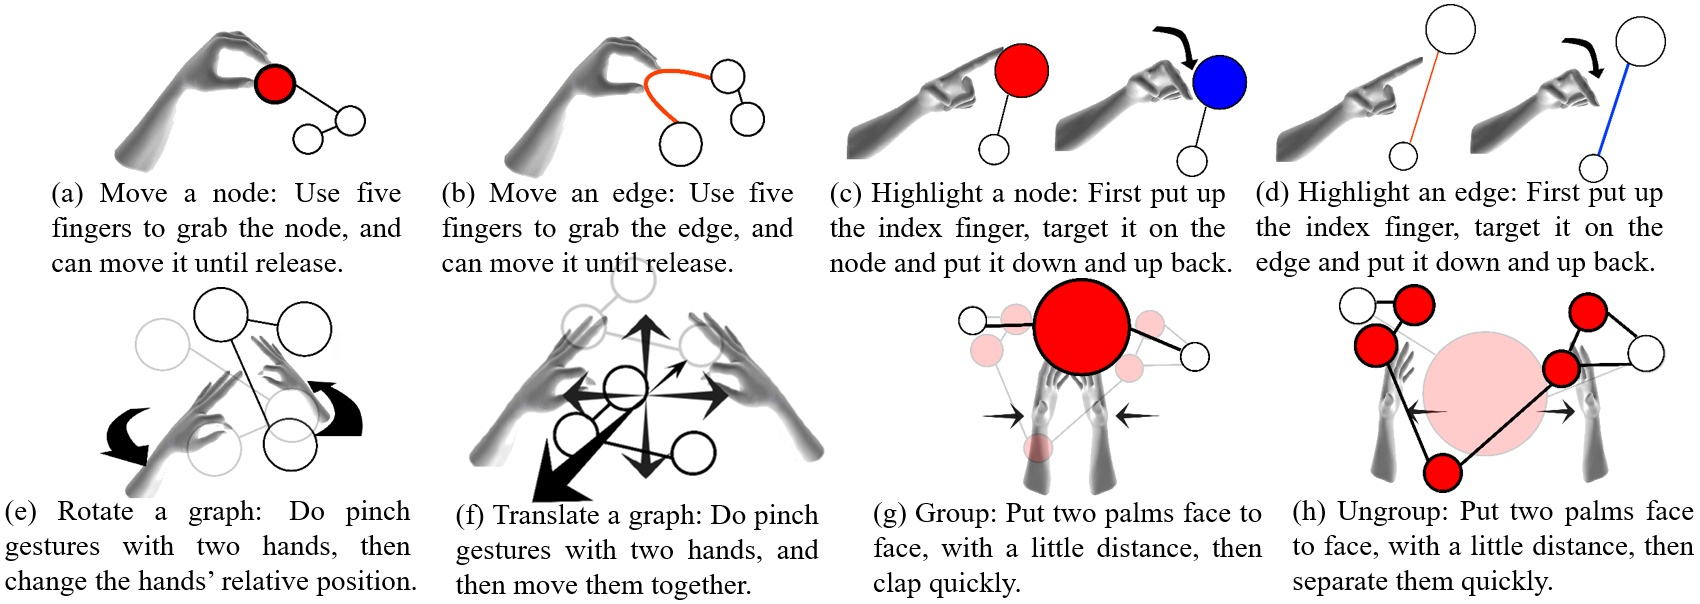
\includegraphics[width=1\textwidth]{graphics/handGestures.jpg}
    \caption{Different possibilities of hand gestures by Yi-Jheng Huang et al. \cite{yi-jheng_huang_gesture_2017}} 
    \label{fig:vrHandGestures} 
\end{figure}

\section{Conclusion}

To design a new visualization, developing a layout concept is one of the first important steps. We summarized some techniques for 2D and 3D visualizations in Section \ref{chap:rw-vrlayouts} and other specially adapted concepts for VR visualizations in Section \ref{chap:rw-2d3dLayout}. In our solution, we combined the explicit and implicit visualization techniques from the 2D and 3D domain, thus creating a unique layout optimized for the use in VR.\\
For navigation, we use the advantage of walking inside the graph we described in Section \ref{chap:rw-vrnavigation} and adapted free-flying and teleportation techniques for further navigation in the scene. Lastly, we apply the ray cast selection described in Section \ref{chap:rw-vrinteraction} to allow selection and interaction.  